\part{Successioni e Serie di Funzioni}
\chapter{Successioni e Serie di Funzioni}
\section{Preliminari}
\definition
Sia $f_n:A\subseteq \R\to \R$ una successione ($n\in\mathbb{N}$) , la serie $\sum\limits_{n=09}^{+\infty}f_n$ indica la successione delle somme parziali $S_n = \sum\limits_{i=0}^nf_i$
\observation
Qualunque affermazione fatta in riferimento ad una serie va quindi intesa riferita alla successione delle somme parziali
\begin{description}
	\item[-] La serie è limitata $\rightleftharpoons$ la successione delle somme parziali è limitata
	\item[-] La serie è illimitata $\rightleftharpoons$ la successione delle somme parziali è illimitata
	\item[-] La serie è convergente $\rightleftharpoons$ la successione delle somme parziali è convergente
\end{description}
\observation
Successioni e serie di funzioni possono essere viste:
\begin{enumerate}
	\item come successioni e serie dipendenti da un parametro
	\item come un mezzo per approssimare funzioni
	\item come un primo passo verso lo studio di funzioni (a volte dette operatori o funzionali) che a funzioni associano o numeri o altre funzioni. 
\end{enumerate}
\section{Tipi Di Convergenza}
\subsection{Convergenza Puntuale}
\definition
Sia $A\subseteq \R$ e $\left\{f_n:n\in\mathbb{N}\right\}$ una successione di funzioni definite su $A$ a valori in $ \R$. Sia $B\subseteq A$
\begin{description}
	\item[-] la successione $\left\{f_n:n\mathbb{N}\right\}$ è puntualmente convergente su $B$ se $\forall x \in B$, esiste finito il limite $\lim\limits_{n\to\infty}f_n(x)$. In tal caso la funzione $f:B\to  \R$ definito da $f(x)=\lim\limits_{n\to\infty}f_n(x)$
	\item[-] la serie $\sum\limits_{n=0}^{\infty}f_n$ è puntualmente convergente su $B$ se $\forall x \in B$, la serie $\sum\limits_{n=0}^{\infty}f_n(x)$ ammette somma finita. In tal caso la funzione $F:B\to  \R$ definito da $F(x)=\sum\limits_{n=0}^{\infty}f_n(x)$ è la somma della serie la serie $\sum\limits_{n=0}^{\infty}f_n$ 
\end{description}
\observation
La convergenza puntuale su $A$ della successione $f_n$ verso $f$ è indicata con
$$f_n\overset{p}{\to}f\quad su A$$
\proposition METAPROPOSIZIONE:\\
Sia $f_n:A\to \R$, $B\subseteq A$, $A\subseteq \R$, $f:B\to A$\\
Se $f_n\overset{p}{\to}f$ su $B$ e se $f_n$ ha la proprietà $P$ allora il limite $f$ ha la proprietà $P$.\\

\example $f_n(x)=\frac{1}{n}sin(x)$ con $A\equiv \R$\\
$\lim\limits_{n\to\infty}f_n(x)=\lim\limits_{n\to\infty}\frac{1}{n}sin(x)=0\quad\forall x \in A \Rightarrow f_n\overset{p}{\to}0$ su $A$.

\example$f_n(x)=e^{nx}$ con $A\equiv \R$
\begin{center}
	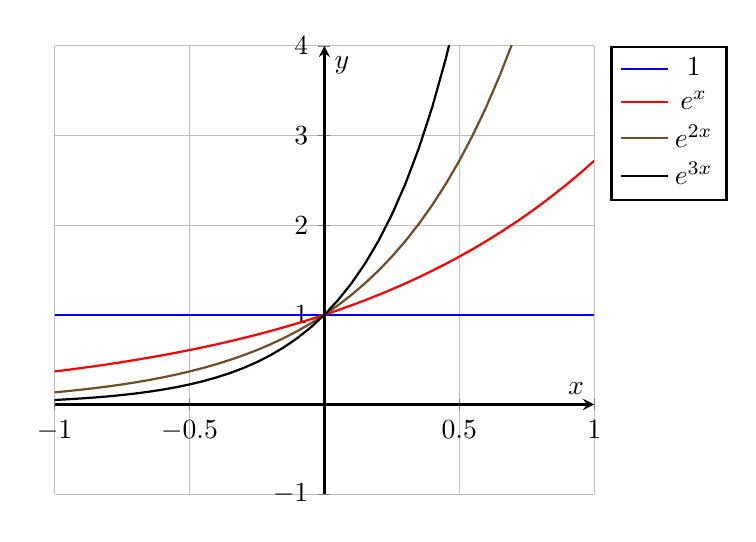
\begin{tikzpicture}[scale=1]
		\begin{axis}[
			xlabel={$x$},ylabel={$y$},
			axis lines=middle,
			samples=41,grid,thick,
			domain=-1:1,
			ymin=-1,ymax=4,
			legend pos=outer north east ]
			\addplot+[no marks] {1}; \addlegendentry{$1$}
			\addplot+[no marks] {e^x}; \addlegendentry{$e^x$} 
			\addplot+[no marks]{e^(2*x)}; \addlegendentry{$e^{2x}$}
			\addplot+[no marks]{e^(3*x)}; \addlegendentry{$e^{3x}$}
			\end{axis}
	\end{tikzpicture}
\end{center}
$$\lim\limits_{n\to\infty}e^{nx} = \left\{\begin{matrix} 0 && x<0\\1&&x=0\\\infty&&x>0 \end{matrix}\right.$$
$$f_n\overset{p}{\to}f\quad su B=\left]-\infty,0\right]$$
\observation
La continuità non passa al limite come proprietà $P$

\example $f_n(x)=x^n$ con $A\equiv \R$
\begin{center}
	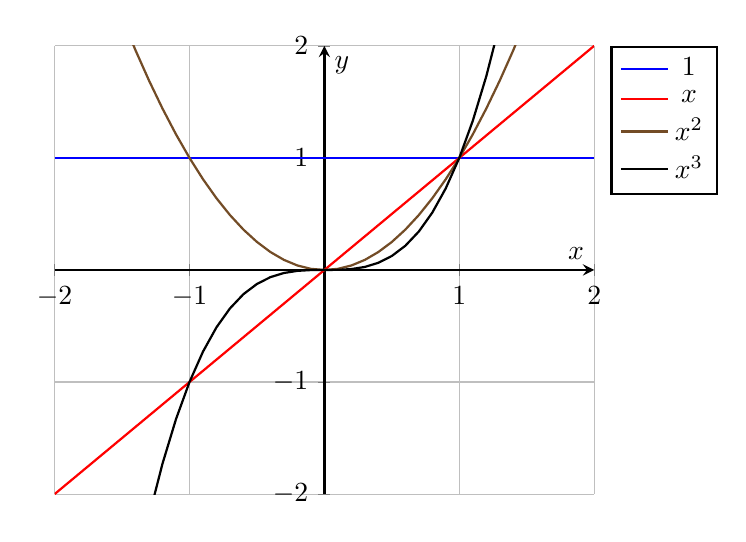
\begin{tikzpicture}[scale=1]
		\begin{axis}[
			xlabel={$x$},ylabel={$y$},
			axis lines=middle,
			samples=41,grid,thick,
			domain=-2:2,
			ymin=-2,ymax=2,
			legend pos=outer north east ]
			\addplot+[no marks] {1}; \addlegendentry{$1$}
			\addplot+[no marks] {x}; \addlegendentry{$x$}
			\addplot+[no marks] {x^2}; \addlegendentry{$x^2$}
			\addplot+[no marks] {x^3}; \addlegendentry{$x^3$}
			\end{axis}
	\end{tikzpicture}
\end{center}
$$\lim\limits_{n\to\infty}x^{n} = \left\{\begin{matrix}+\infty&&x\in\left]1,+\infty\right[\\ 1 && x\in\left\{1\right\}\\0&&x\in\left]-1,1\right[\\\nexists &&x\in\left]-\infty,-1\right] \end{matrix}\right.$$
$$f_n\overset{p}{\to}f\quad su B=\left]-1,1\right]$$
\proposition PROPRIETÀ P:MONOTONIA\\
Sia $f_n:A\to \R$, $B\subseteq A$, $A\subseteq \R$, $f:B\to A$\\
Se $f_n\overset{p}{\to}f$ su $B$ e se $f_n$ è debolmente crescente su $B$ allora il limite $f$ è debolmente crescente su $B$.
\begin{proof}
	Dire che $f_n$ è debolmente crescente su $B$ significa che $$\forall x_1,x_2\in B \quad x_1\le x_2 \Rightarrow fn(x_1)\le f_n(x_2)$$
	se si fa tendere $n\to\infty$ si ha che $f(x_1)\le f(x_2)$, e questo nell'insieme $B$ dove i limiti puntuali delle funzioni esistono per ipotesi
\end{proof}
\observation
Questo vale anche nel caso di funzioni debolmente decrescenti
\observation
se $f_n$ è strettamente crescente/decrescente con le stesse ipotesi non possiamo concludere che il limite puntuale mantenga la stessa proprietà\\
\example $x^n$ con $x\in\left[0,1\right[$ è strettamente crescente ma il limite putuale è costante uguale a zero.
\proposition PROPRIETÀ P:NON NEGATIVA\\
Sia $f_n:A\to \R$, $B\subseteq A$, $A\subseteq \R$, $f:B\to A$\\
Se $f_n\overset{p}{\to}f$ su $B$ e se $f_n$ è non negativa, $f_n\ge 0$, su $B$ allora il limite $f$ è non negativo, $f\ge 0$, su $B$.
\begin{proof}
 	Sappiamo che $f(x)=\lim\limits_{n\to\infty}f_n(x)$ $\forall x\in B$.
 	Ma $f_n$ è una successione di valori non negativi quindi il limite esiste ed è non negativo.
\end{proof}
\observation
Questo vale anche nel caso di funzioni non positive
\observation
Questa proposizione non può essere estesa al caso di funzioni strettamente positive/negative.\\
\example $	-\frac{e^x}{n}$ con $x\in\left[0,1\right[$ è strettamente negativa ma il limite è costante uguale a zero.
\proposition
Siano $A\subseteq \R, B\subseteq A$, $\left\{f_n:n\in\mathbb{N}\right\}$ una successione di funzioni definite su $A$ con valori in $ \R$. sia $f:B\to \R$ una funzione\\
$f_n\overset{p}{\to}f$ su $B$ per $n\to\infty \Leftrightarrow \forall x\in B,\forall \epsilon >0,\exists\nu\in\mathbb{N}:\forall n>\nu \quad \abs{f_n(x)-f(x)}\le \epsilon$
\begin{proof}
	direttamene dalla definizione...
\end{proof}
\proposition
Siano $A\subseteq \R, B\subseteq A$, $\left\{f_n:n\in\mathbb{N}\right\}$ una successione di funzioni definite su $A$ con valori in $ \R$. Sia $F:B\to \R$ una funzione\\
$\sum\limits_{n=0}^{\infty}f_n\overset{p}{\to}F$ su $B$ per $n\to\infty \Leftrightarrow \forall x\in B,\forall \epsilon >0,\exists\nu\in\mathbb{N}:\forall n>\nu \quad \abs{\sum\limits_{k=0}^{\infty}f_k(x)-F(x)}\le \epsilon$
\begin{proof}
	direttamene dalla definizione...
\end{proof}

\subsection{Convergenza Uniforme}
\definition
Siano $A\subseteq \R$, $B\subseteq A$, $\left\{f_n:n\in\mathbb{N}\right\}$ una successione di funzioni definite su $A$ a  valori in $ \R$.
\begin{description}
	\item[-] La successione $\left\{f_n:n\in\mathbb{N}\right\}$ è uniformemente convergente su $B$ se esiste una funzione $f:B\to \R$ t.c.:
	$$\lim\limits_{n\to\infty} \sup\limits_{x\in B}\abs{f_n(x)-f(x)}=0$$
	la funzione $f$ è il limite uniforme della successione $fn$
	\item[-] La serie $\sum\limits_{n=0}^{\infty}f_n$ è uniformemente convergente su $B$ se esiste una funzione $F:B\to \R$ t.c.:
	$$\lim\limits_{n\to\infty} \sup\limits_{x\in B}\abs{F(x)-\sup\limits_{n=0}f_n(x)}=0$$
	la funzione $F$ è il limite uniforme della serie $\sum\limits_{n=0}^{\infty}f_n$ 
\end{description}
\observation
La convergenza uniforme su $B$ della successione $f_n$ verso $f$ è indicata con
$$f_n\overset{u}{\to}f\quad su \quad B$$
\begin{observation}
	\label{obs:dist_conv_unif}
	la convergenza uniforme equivale alla convergenza rispetto alla distanza $d_{\cntclass{0}}(f,g)=\sup\limits_{x\in A}\abs{g(x)-f(x)}$ ogniqualvolta questa distanza sia definita.\\
	Questa distanza $d_{\cntclass{0}}(f,g)$ può essere definita attraverso la norma $\norm{k}_{\cntclass{0}}=\sup\limits_{x\in A}\abs{k}$ con $k = f-g$
\end{observation}
\proposition
sia $f_n:n\in\mathbb{N}$ con $f:A\subseteq \R\to \R$ e $f:B\subseteq A \to  \R$\\
$f_n\overset{u}{\to}f$ su $B$ per$n\to\infty \Leftrightarrow \forall\epsilon >0, \exists\nu\in\mathbb{N}$  t.c: $\forall n>\nu, \forall x\in B$ vale che $\abs{f_n(x)-f(x)}\le\epsilon$
\proposition
sia $f_n:n\in\mathbb{N}$ con $f:A\subseteq \R\to \R$ e $F:B\subseteq A \to  \R$\\
$\sum\limits_{n=0}^{\infty}f_n\overset{u}{\to}F$ su $B\Leftrightarrow \forall\epsilon >0, \exists\nu\in\mathbb{N}$  t.c: $\forall n>\nu, \forall x\in B$ vale che $\abs{F(x)-\sum\limits_{k=0}^{n}f_k(x)}\le\epsilon$
\observation
La differenza tra queste due proposizioni e le due proposizioni analoghe nel caso di convergenza puntuale giustifica il fatto che la continuità non passa al limite puntuale. Infatti qui $\nu$ dipende solo dalla scelta di $\epsilon$ e le $x$ si guardano tutte insieme, prima invece $\nu$ dipendeva oltre che alla $\epsilon$ anche dalla $x$ questo porta a osservare le $x$ una alla volta.
\proposition Relazione tra convergenza uniforme e puntuale.\\
Sia $f_n:A\subseteq \R\to \R$ e $f:B\subseteq A\to \R$\\
Se $fn\overset{u}{\to}f$ su $B$ allora $fn\overset{p}{\to}f$ su $B$.
\begin{proof}
	se $f_n\overset{u}{\to}f$ su $b$ allora vale che:
	$\forall\epsilon, \exists\nu : \forall n>\nu, \forall x\in B $ vale $\abs{f_n(x)-f(x)}\le\epsilon$ in questo modo si trova un $\nu$ che soddisfa la condizione $\forall x \in B$ quindi $\forall x\in B, \forall\epsilon, \exists\nu : \forall n>\nu $ vale $\abs{f_n(x)-f(x)}\le\epsilon$ quindi $f_n\overset{p}{\to}f$ su B
\end{proof}
\proposition
Sia $f_n:A\subseteq \R\to \R$ e $\overline{f},f:B\subseteq A\to \R$\\
se $f_n\overset{u}{\to}f$ su $B$ e $f_n\overset{u}{\to}\overline{f}$ su $B$ allora $f=\overline{f}$
\begin{proof}
	$f_n\overset{u}{\to}f$ e $f_n\overset{u}{\to}\overline{f}$, quindi è anche vero che $f_n\overset{p}{\to}f$ e $f_n\overset{p}{\to}\overline{f}$ ma il limite puntuale è unico poichè è il limite di una successione. Allora $f=\overline{f}$
\end{proof}
\example $f_n(x)=\frac{1}{n}sin(x)$ con $A\equiv \R$\\
Abbiamo gia calcolato che $f_n\overset{p}{\to}0$ su $A$.\\
Sia ha anche convergenza uniforme :\\
$$\lim\limits_{n\to\infty}\sup{ \R}\abs{f_n(x)-0} = \lim\limits_{n\to\infty}\sup\limits_{ \R}\abs{\frac{1}{n}sin(x)}$$
Osservo che $\abs{asin(x)}\le\abs{a}$ quindi 
$$\lim\limits_{n\to\infty}\sup\limits_{ \R}\abs{\frac{1}{n}sin(x)}\le\lim\limits_{n\to\infty}\frac{1}{n}=0$$
Allora $f_n\overset{u}{\to}f$ su $A$

\example $f_n(x)=sin\left(\frac{1}{n}x\right)$ con $A\equiv \R$
..........\\
..........\\
\proposition
Siano $A\subseteq \R$, $\left\{f_n:A\to \R:n\in\mathbb{N}\right\}$ una successione di funzioni e $f:A\to \R$\\
$f_n\overset{u}{\to}f$ su $A$ e $f_n\in \cntclass{0}(A; \R)\,\,\forall n\in\mathbb{N}$ allora $f\in \cntclass{0}(A; \R)$
\begin{proof}
	DISEGNO\\
	DISEGNO\\
	DISEGNO\\
	DISEGNO\\
	GIURO CHE LA FAROò
	(a distanza di tre anni non son sicurissimo che lo farò)
\end{proof}
\example $f_n(x)=\sqrt{x^2+\frac{1}{n}}$ con $A\equiv \R$\\
%$f_n$ è continua $\forall n$ perchè compositione di funzioni continue.\\
%Il limite puntuale di questa successione di funzioni è $f\left( x \right)=\abs{x}$ su $A$\\
%Si può verificare che $f\left(x\right)=\abs{x}$ è anche limite uniforme su $A$ poichè
%$$ \lim\limits_{n\to\infty}\sup\limits_{x\in A} \abs{\sqrt{x^2+\frac{1}{n}}-\left|x}\right| $$
%analizzando il contenuto del modulo si trova che la sua derivata vale $\frac{1}{2\sqrt{x^2+\frac{1}{n}}}-sgn\left(x\right)$ che si annulla in $x=\pm\sqrt{\frac{1}{4}-\frac{1}{n}}$
..........\\
..........\\
\definition
Siano $A\subseteq \R$, $B\subseteq A$ e $\left\{f_n:A\to \R:n\in\mathbb{N}\right\}$ una successione di funzioni.\\
La successione $\left\{f_n:n\in\mathbb{N}\right\}$ soddisfa alla condizione di Cauchy per la convergenzauniforme su $B \rightleftharpoons \forall\epsilon>0, \exists\nu\in\mathbb{N}: \forall n,m>\nu, \forall x \in B$ vale $\abs{f_n(n)-f_m(x)}<\epsilon$
\proposition
(Una successione di Cauchy per la convergenza uniforme è uniformemente convergente).\\
Siano $A\subseteq \R$, $B\subseteq A$ e $\left\{ f_n:A\to \R:n\in\mathbb{N} \right\}$ una successione di funzioni.\\
La successione $\left\{ f_n:n\in\mathbb{N} \right\}$ soddisfa alla condizione di Cauchy per la convergenza uniforme su $B$ allora $\exists$ una funzione $f:B\to \R$ t.c.: $f_n\overset{u}{\to}f$ su $B$
\begin{proof}
	La successione $\left\{ f_n:n\in\mathbb{N}\right\}$ soddisfa alla condizione di Cauchy per la convergenza uniforme su $B$ allora $\forall x\in B$ la successione $\left\{ f_n(x) :n\in\mathbb{N} \right\}$ è di Cauchyin $ \R$ allora $\forall x \in B$ la successione $\left\{ f_n(x):n\in\mathbb{N} \right\}$ ha limite in $ \R$.(cioè c'è il limite puntuale).\\
	Sia $f(x)$ questo limite, $f$ è anche il limite uniforme della successione $\left\{ f_n:n\in\mathbb{N} \right\}$, infatti:
	$$\forall\epsilon>0, \exists\nu\in\mathbb{N}: \forall h,k>\nu \forall x\in B \quad \abs{f_h-f_k}<\epsilon$$
	$$\sup\limits_B\abs{f_h(x)-f_k(x)}, \forall h,k>\nu$$
	$$\Rightarrow \abs{f_h(x)-f_k}<\epsilon,\forall h.k>\nu, \forall x \in B$$
	a questo punto si passa al limite e la disuguaglianza diventa debole.
	$$\Rightarrow \lim\limits_{n\to\infty}\abs{f_h(x)-f_k(x)}\le\epsilon, \forall h>\nu, \forall x\in B$$
	$$\Rightarrow\abs{f_h(x)-f(x)}\le\epsilon, \forall h>\nu, \forall x\in B$$
	$$\Rightarrow\sup\limits_B\abs{f_h-f}\le\epsilon, \forall h>\nu$$
	$$\Rightarrow f_n\overset{u}{\to}f\quad su B$$
\end{proof}
\begin{proposition}
	Sia $A$ un compatto in $ \R$. In $\cntclass{0}(A; \R)$ sia $d_{\cntclass{0}}=\sup_A\abs{g(x)-f(x)}$. Allora $\left( \cntclass{0}\left(A; \R\right);d_{\cntclass{0}}\right)$ è uno spazio metrico completo.
	\begin{proof}
		prendo $f_n\in \cntclass{0}(A; \R)$ successione di Cauchy in $\cntclass{0}(A; \R)$
		$f_n$ sono di Cauchy rispetto alla convergenza uniforme su $A$
		$\Rightarrow f_n:A\to \R$ e $f_n\overset{u}{\to}f$ su $A$ e $f$ è continua\\ $\Rightarrow\left(f\in \cntclass{0}(A; \R)\right)$\\
		$\Rightarrow\lim\limits_{n\to\infty}f_n=f$ in $\cntclass{0}(A; \R)$\\
		$\Rightarrow\lim\limits_{n\to\infty}d_{\infty}(fn,f)=0\quad\Rightarrow f_n\to f\in \cntclass{0}(A; \R)$
	\end{proof}
\end{proposition}
\begin{corollary} % TODO dimostrare il corollario 19.26 con C di arrivo delle f chiuso
	\label{prop:compl_dist_spm_compl}
\end{corollary}

ESEMPIO:: In dimensione finita non vi è differenza tra "chiuso e limitato" e "compatto", in dimensione infinita cambiamo molte cose.
Prensiamo un insieme chiuso e limitato ma non compatto.\\
In $\cntclass{0}(\left[0,1\right]; \R)$ con $d_\infty(f,g)=\sup_{\left[0,1\right]}\abs{g(x)-f(x)}$, prendiamo l'insieme $C=\overline{B(0,1)}=\left\{f\in \cntclass{0}(\left[0,1\right]; \R):\abs{f(x)}\le 1, \forall x \in\left[0,1\right]\right\}$
\begin{description}
	\item[1] $C$ è limitato: ha diametro finito.
	\item[2] $C$ è chiuso: contiene tutti i sui punti di accumualazione
\end{description}
Se c'è una successione $f_n\overset{u}{\to}f$ su $\left[0,1\right]$ allora voglio mostrare che $f\in C$\\
Se $f_n\overset{u}{\to}f$ su $\left[0,1\right]$ allora $f_n\overset{p}{\to}f$ su $\left[0,1\right]$.
Sappiamo che $\forall n\in\mathbb{N}$ e $\forall x\in \left[0,1\right]$ vale che $-1\le f_n(x)\le 1$.\\
Mandando $n$ al limite si ha che $-1\le f_(x)\le 1$.\\
Inolte $f$ è continua perché limite uniforme di una successione di funzioni continue allora $f\in C$ poiché è una funzione continua compresa tra $-1$ e $1$
\begin{description}
	\item[3] $C$ non è compatto, cioè esiste almeno una successione dalla quale non è possibie estrarre una sottosuccessione convergente nello stesso spazio.
\end{description}
Se ad esempio $f_n(x) = x^n$\\
so che $f_n\overset{p}{\to}f$ su $\left[0,1\right]$ e $f(x)=\left\{\begin{matrix}0&&x\in\left[0,1\right]\\1&&x\in\left\{1\right\}\end{matrix}\right.$\\
Tutta la successione di funzioni $f_n$ converge puntualmente a $f$ quindi se estraggo una sottosuccessione comunque venga scelta questa sottosuccessione converge ancora a $f$ puntualmente. Ma la $f$ non è continua mentre il limite uniforme di funzioni continue è una funzione continua allora nessuna sottosuccessione ammette limite uniforme.\\

ESEMPIO:: OPERATORE DERIVATA 0\\
$$D$$

ESEMPIO:: OPERATORE DERIVATA 1\\
$$D$$

ESEMPIO:: OPERATORE INTEGRALE\\
$$I$$

\proposition
fissati $a,b\in \R$ con $a<b$ se la successione $\left\{f_n:n\in\mathbb{N}\right\}$ in $\cntclass{0}(\left[a,b\right], \R)\overset{u}{\to}f$ su $\left[a,b\right]$\\
$f_n$ e $f$ sono integrabili secondo Rimmmmmmmn allora lasuccessione $\left\{\int_a^bf_n(x)\integrald{x}:n\in\mathbb{N}\right\}$ converge a $\int_a^bf(x)\integrald{x}$
\observation
La convergenzauniforme passa sotto il segno di integrale 
$$\int_a^b\left(\lim\limits_{n\to\infty}fn\right)(x)\integrald{x}=\lim\limits_{n\to\infty}\left(\int_a^bfn(x)\integrald{x}\right)$$
\proposition convergono le derivare allora convergono le funzioni\\
Fissati $a,b\in \R$ con $a<b$, si consideri una successione di funzioni $\left\{f_n:n\in\mathbb{N}\right\}$ con $f_n:\left[a,b\right]\to \R$
\begin{enumerate}
	\item $\forall n\in\mathbb{N}, f_n\in \cntclass{1}(\left[a,b\right]; \R)$
	\item $\exists x_0\in\left[a,b\right]: \lim\limits_{n\to\infty}f_n(x_0)=l\in \R$
	\item $\exists g \in \cntclass{0}(\left[a,b\right]; \R):f'_n\overset{u}{\to}g$ su $\left[a,b\right]$
\end{enumerate}
Allora
\begin{enumerate}
	\item $\exists f\in \cntclass{1}(\left[a,b\right]; \R)$
	\item $f_n\overset{u}{\to}f$ su $\left[a,b\right]$
	\item $f'(x)=g(x)$ $\forall x\in\left[a,b\right]$
\end{enumerate}
\begin{proof}
	Per il teorema fondamentale del calcolo integrale
	$$f_n(x)=f_n(x_0)+\int_{x_0}^{x}f_n'(t)\integrald{t}$$
	per $n\to\infty$
	$$f(x)=l+\int_{x_0}^{x}g(t)\integrald{t}$$
	Quindi le $f_n$ convergono puntualmente alla funzione $f(x)$, per la convergenza uniforme calcolo:
	$$ \lim\limits_{n\to+\infty}\sup\limits_{\left[a,b\right]}\abs{f_n(x)-f(x)}\le\lim\limits_{n\to+\infty}(\abs{f_n(x_0)-f(x_0)}+\abs{\int_{x_0}^x \abs{f_n'(t)-g(t)}\integrald{t}})\le$$
	$$\lim\limits_{n\to+\infty}\left[ \abs{f_n(x_0)-f(x_0)}+\abs{b-a}\sup\limits_{\left[a,b\right]}\abs{f_n'(x)-g(x)} \right] = $$
	Questo perché per ipotesi $f'_n=g$ e il limite fa $0$.
	Allora $f_n\overset{u}{\to}f$ su $\left[a,b\right]$\\
	Inoltre si sa che $f_n\in \cntclass{1}$ allora $f_n'\in \cntclass{0}$ allora il limite uniforme di funzioni continue è una funzione continua allora $g$ è una funzione continua.\\
	La $f$ è l'integrale di una funzione continua allora la $f$ è derivabile con derivata continua quindi $f'=g$
\end{proof}
\observation
Necessaria l'ipotesi $f_n(x_0)\to l$.......
\observation
Serve $\left[a,b\right]$ limitato .......\\
.............................\\
................................\\
\proposition
Fissati $a,b\in \R$ con $a<b$, si consideri una successione di funzioni $\left\{f_n:n\in\mathbb{N}\right\}$ con $f_n:\left[a,b\right]\to \R$
\begin{enumerate}
	\item $\forall n\in\mathbb{N}, f_n\in \cntclass{1}(\left[a,b\right]; \R)$
	\item $\exists x_0\in\left[a,b\right]: \sum\limits_{n=0}^{+\infty}f_n(x_0)=L\in \R$
	\item $\exists g \in \cntclass{0}(\left[a,b\right]; \R): \sum\limits_{n=0}^{+\infty}f_n\overset{u}{\to}g$ su $\left[a,b\right]$
\end{enumerate}
Allora
\begin{enumerate}
	\item $\exists f\in \cntclass{1}(\left[a,b\right]; \R)$
	\item $\sum\limits_{n=0}^{+\infty}f_n\overset{u}{\to}f$ su $\left[a,b\right]$
	\item $f'(x)=g(x)$ $\forall x\in\left[a,b\right]$
\end{enumerate}
\observation
In altre parole questa proposizione afferma che sotto opportune ipotesi
$$\left(\sum\limits_{n=0}^{+\infty} f_n \right)' =  \sum\limits_{n=0}^{+\infty}f_n'$$
\definition
Siano $A\subseteq  \R$ e $\left\{f_n:n\in\mathbb{N}\right\}$ una successione di funzioni con $f_n:A\to \R$\\
$\sum\limits_{n=0}^{+\infty}f_n$ converge totalmente su $A \rightleftharpoons \sum\limits_{n=0}^{+\infty}\sup\limits_{A}\abs{f_n(x)}<+\infty$(è convergente) 
\observation
la $\sum\limits_{n=0}^{+\infty}\sup\limits_{A}\abs{f_n(x)}$ è una serie numerica
\proposition
Siano $A\subseteq \R$ e $\left\{f_n:n\in\mathbb{N}\right\}$ una successione di funzioni con $f_n:A\to \R$\\
$\sum\limits_{n=0}^{+\infty}f_n$ converge totalmente su $A$ $\Rightarrow$  $\sum\limits_{n=0}^{+\infty}f_n$ converge uniformemente su $A$
\begin{proof}
	$\sum\limits_{n=0}^{+\infty}f_n$ converge totalmente su $A$\\
	$\Rightarrow \sum\limits_{n=0}^{+\infty}\sup\limits_{x\in A}\abs{f_n(x)}<+\infty$\\
	$\Rightarrow \forall\epsilon>0, \exists\nu\in\mathbb{N}: \forall n,m\in\mathbb{N}$ con $m>n>\nu$ vale $\sum\limits_{n=0}^{+\infty}\sup\limits_{x\in A}\abs{f_n}<\epsilon$\\
	$\Rightarrow \forall\epsilon>0, \exists\nu\in\mathbb{N}: \forall n,m\in\mathbb{N}$ con $m>n>\nu$ vale $\sup\limits_{x\in A}\sum\limits_{n=0}^{+\infty}\abs{f_n}<\epsilon$\\
	$\Rightarrow \forall\epsilon>0, \exists\nu\in\mathbb{N}: \forall n,m\in\mathbb{N}$ con $m>n>\nu$ vale $\sup\limits_{x\in A}\abs{\sum\limits_{n=0}^{+\infty}f_n}<\epsilon$\\
	$\Rightarrow \sum\limits_{n=0}^{+\infty}f_n$ soddisfa la condizione di Cauchy per la convergenza uniforme su $A$.
\end{proof}
\observation
Per le serie:\\
Convergenza Totale $\Rightarrow$ Convergenza Uniforme $\Rightarrow$ Convergenza Puntuale.

\section{Serie di Funzioni Particolari}
Questa sezione è dedicata ad alcune tecniche di approssimazione  basate su serie di funzioni particolari\\
In generale, un'approssimazione si riconduce ad una formula del tipo\\
$$\left[\text{quantità da calcolare}\right]=\left[\text{quantità approssimante}\right]+ errore$$
La qualità dell'approssimazione è descritta dal senso in cui l'errore è piccolo.\\
\subsection{Serie di Potenze}
\definition
Siano $\left\{a_n:n\in\mathbb{N}\right\}$ una successione con $a_n:\mathbb{N}\to\mathbb{C}$ e $z_0\in\mathbb{C}$.\\
Si dice serie di potenze centrata in $z_0 \rightleftharpoons \sum\limits_{n=0}^{+\infty}a_n\left(z-z_0\right)^n$ 
\observation
è ovvio che in $z=z_0$ si ha convergenza....???? (dire a zero)
\observation
Per semplicità verrà considerato il caso $z_0=0$
ESEMPIO::$\sum\limits_{n=0}^{+\infty}\frac{x^n}{n!}=1+x+\frac{1}{2} x^2+\ldots+\frac{1}{n!}x^n=e^x$ 
ESEMPIO::$\sum\limits_{n=0}^{+\infty}x^n=1+x+x^2+\ldots+x^n=\frac{1}{1-x}$
\proposition
Siano $\left\{a_n:n\in\mathbb{N}\right\}$ una successione in $\mathbb{C}$ e $w\in\mathbb{C}$.\\
La serie di potenze $\sum\limits_{n=0}^{+\infty}a_nz^n$ converge in $w$ (cioè $\sum\limits_{n=0}^{+\infty}a_nw^n$ converge) quandi abbiamo la convergenza nella sfera aperta di centro l'origine e raggio $\abs{w}$\\
Allora $\forall r$ con $0<r<\abs{w}$, la serie di potenze $\sum\limits_{n=0}^{+\infty}a_nz^n$ converge totalmente in $B(0,r)$\\
\begin{proof}
	TIKZPICTURE:::::\\
	devo dimostrare che $\sum\limits_{n=0}^{+\infty}\sup\limits_{B(0,r)}\abs{a_nz^n}<+\infty$.\\
	E\' facile vedere che $a_nz^n=a_nw^n\left(\frac{z}{w}\right)^n$.\\
	Quindi passando al modulo e poi al sup si ottiene.\\
	$$\sup\limits_{B(0,r)}\abs{a_nz^n}=\sup\limits_{B(0,r)}\abs{a_nw^n}\abs{\frac{z}{w}}^n\le$$
	Siccome $\sum\limits_{n=0}^{+\infty}a_nw^n$ converge  quindi il suo termine generale tende a $0$.\\
	$$\le\sup\limits_{B(0,r)}\abs{\frac{z}{w}}^n\le\left(\frac{r}{\abs{w}}\right)^n $$
	per ipotesi $r<\abs{w}$ e questo è il termine generale di una serie geometrica convergente.\\
	Ne segue che $\sum\limits_{n=0}^{+\infty}\sup\limits_{B(0,r)}\abs{a_nz^n}$ è maggiorato da $\left( \frac{r}{\abs{w}}\right)^n$ e quindi la serie converge totalmente.
\end{proof}
\observation
Una volta che abbiamo la convergenza totale abbiamo anche quella uniforme.
\proposition la non convergenza in un punto implica la non convergenza fuori dal cerchio\\
Sia ${a_n:n\in\mathbb{N}}$ una successione a valori in $\mathbb{C}$\\
La serie $\sum\limits_{n=0}^{+\infty}a_nz^n$ non  converge in $w$\\
Allora $\forall z\in\mathbb{C}$ con $\abs{z}>\abs{w}$ la serie di potenze $\sum\limits_{n=0}^{+\infty}$ non converge in $z$
\begin{proof}
	\begin{center}
		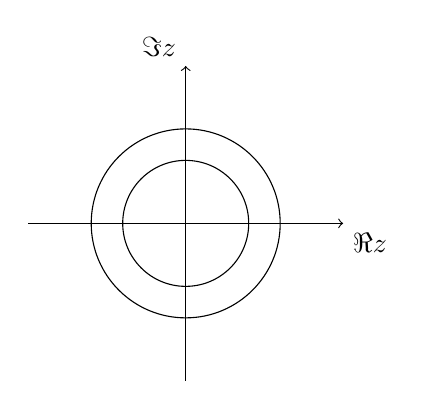
\begin{tikzpicture}[scale=1]
		\draw[->] (-2,0) -- (2,0) node[anchor=north west] {$\Re{z}$};
		\draw[->] (0,-2) -- (0,2) node[anchor=south east] {$\Im{z}$};
		\clip (-2,-2) rectangle (2,2);
		\draw (0,0) circle (1.2cm);
		\draw (0,0) circle (0.8cm);
		\end{tikzpicture}
	\end{center}
	Se per assurdo la serie converge in $z\Rightarrow$ per il teorema precedente  avremmo convergenza in ogni sfera con raggio minore di $\abs{\frac{1}{z}}$. e quindi anche in $w$ questo nega l'ipotesi.ASSURDO.
\end{proof}
\observation
Come è fatto l'insieme su cui si ha convergenza??\\
segue da queste due ultime proposizioni che se $\left\{a_n:n\in\mathbb{N}\right\}$ è una successione in $\mathbb{C}$ allora l'insieme $\left\{z\in\mathbb{C}:\sum\limits_{n=0}^{+\infty}a_nz^n converge\right\}$ è un cerchio.\\Sulla circonferenza non ci soffermaiamo a capire cosa accade poiché tutto può accadere.
\definition
Raggio di convergenza della serie $\sum\limits_{n=0}^{+\infty}a_nz^n\rightleftharpoons \rho=\sup\left\{r\ge 0 :\sum\limits_{n=0}^{+\infty}a_nz^n converge su B(0,r)\right\}$
\observation
Il raggio di convergenza di una serie di potenze può essere $0$, un numero reale positivo o $+\infty$.
\observation
una definizione come $\rho=\inf\left\{r\ge 0 :\sum\limits_{n=0}^{+\infty}a_nz^n non converge su B(0,r)\right\}$ non sta in piedi poiché questo insieme potrebbe essere vuoto, mentre quello sopra non è mai vuoto, poerché $r=0$ c'è sempre poiché in $0$ si ha sempre convergenza. Ilsecondo potrebbe essere vuoto perché ci sono serie che convergono su tuttoil piano complesso e quindi non si avrebbe nessun $r$ fuori da quale non sia ha convergenza.\\
\proposition CRITERIO DELLA RADICE.\\
Data la serie di potenze $\sum\limits_{n=0}^{+\infty}a_nz^n$, sia $l=\lim\limits_{n\to+\infty}\sqrt[n]{\abs{a_n}}$.\\
Se questo limite esiste, allora il raggio di convergenza è 
$\rho =
	\begin{cases}
		0				&	\text{se }l=+\infty\\
		\frac{1}{l} 	&	\text{se }l\in\left]0,+\infty\right[\\
		+\infty 		& 	\text{se }l=0
	\end{cases}
$
\proposition CRITERIO DEL RAPPORTO.\\
Data la serie di potenze $\sum\limits_{n=0}^{+\infty}a_nz^n$, sia $l=\lim\limits_{n\to+\infty}\frac{a_{n+1}}{a_n}$.\\
Se questo limite esiste, allora il raggio di convergenza è 
$\rho =
\begin{cases}
0				&	\text{se }l=+\infty\\
\frac{1}{l} 	&	\text{se }l\in\left]0,+\infty\right[\\
+\infty 		& 	\text{se }l=0
\end{cases}
$
ESEMPIO::$e^z=\sum\limits_{n=0}^{+\infty}\frac{1}{n!}z^n$\\
$a_n=\frac{1}{n!} ...  \abs{\frac{a_{n+1}}{a_n}}=\frac{\frac{1}{(n+1)!}}{\frac{1}{n!}}=\frac{n!}{(n+1)!}=\frac{1}{n+1}\overset{n\to+\infty}{\to}0 \Rightarrow \rho=+\infty$\\
ESEMPIO::$sin(z)=\sum\limits_{n=0}^{+\infty}\frac{(-1)^nz^{2n+1}}{(2n+1)!}$ quindi 
$a_n =
\begin{cases}
0		&	\text{se }n\text{ è pari}\\
...		&	\text{se }n\text{ è dispari}\\
\end{cases}
$\\
...\\
...\\
...\\
ESEMPIO::$sin(z)=\sum\limits_{n=0}^{+\infty}\frac{(-1)^nz^{2n}}{(2n)!}$ quindi 
$a_n =
\begin{cases}
...		&	\text{se }n\text{ è pari}\\
0		&	\text{se }n\text{ è dispari}\\
\end{cases}
$\\
...\\
...\\
...\\
ESEMPIO:: $e^{iy}$ con $y\in \R$ 
$$e^{iy} = \sum\limits_{n=0}^{+\infty}\frac{1}{n!}(iy)^n = \sum\limits_{n=0}^{+\infty}\frac{1}{(2n)!}(iy)^{2n} + \sum\limits_{n=0}^{+\infty}\frac{1}{(2n+1)!}(iy)^{2n+1} = $$
$$ = \sum\limits_{n=0}^{+\infty}\frac{(-1)^n}{(2n)!}(y)^{2n} + i\sum\limits_{n=0}^{+\infty}\frac{(-1)^n}{(2n+1)!}(y)^{2n+1} = cos(y)+isin(y)$$
\begin{enumerate}
	\item $i^{2n}=\left(i^2\right)^n=(-1)^n$
	\item $i^{2n+1}=i\left(i^2\right)^n=i(-1)^n$
\end{enumerate}
ESEMPIO:: $e^{i\pi}+1=cos(\pi)+i\cdot sin(\pi)=0$\\
ESEMPIO:: $\sum\limits_{n=0}^{+\infty}z^n=\frac{1}{1-z}$ con $\rho=1$
ESEMPIO:: Sia $f(x)=\frac{1}{1+x^2}=\frac{1}{1-(-x^2)} = \sum\limits_{n=0}^{+\infty}(-x^2)^n=\sum\limits_{n=0}^{+\infty}(-1)^nx^{2n}$\\
QUI GRAFICO ..............\\
..........................\\
Questa serieconverge esclusivamente per $\abs{x}<1$, mentre la funzione $f$ è definita su tutto $ \R$, $f\in \cntclass{\infty}( \R; \R)$\\
In $\mathbb{C}$, lafunzione $f(z)=\frac{1}{1+z^2}$ è la somma della serie $\sum\limits_{n=0}^{+\infty}(-1)^nz^{2n}$ che ha raggio di convergenza  $\rho=1$. Infatti, $f(z)$ è singolare sia in $z=i$ sia in $z=-i$.\\
ALTRO GRAFICO::::::::::::::::\\
................................\\

\subsection{Serie di Taylor}
ESEMPIO:: $ln(1+z)$. Calcolare la Serie di Taylor.\\
$$D\left[ln(1+z)\right] = \frac{1}{1+z} = \sum\limits_{n=0}^{+\infty}(-1)^nz^n$$
$$\int \sum\limits_{n=0}^{+\infty}(-1)^nz^n dz = \sum\limits_{n=0}^{+\infty}\frac{(-1)^n}{n+1}z^{n+1}=\sum\limits_{n=1}^{+\infty}\frac{(-1)^{n-1}}{n}z^n$$
\proposition
Sia $\left\{a_n:n\in\mathbb{N}\right\}$ una successione a valori in $\mathbb{C}$. Le serie:
\begin{center}
	$\left.\begin{matrix}
	
	\ast&&\sum\limits_{n=0}^{+\infty}a_nz^n\\
	\ast&&\sum\limits_{n=0}^{+\infty}na_nz^{n-1}\\
	\ast&&\sum\limits_{n=0}^{+\infty}\frac{a_n}{n+1}z^{n+1}\\
	
	\end{matrix}\right\}$ hanno lo stesso raggio di convergenza
\end{center}

\definition
Sia $r\in \R$ con $r>0$. La funzione $f$ si dice analitica su $\left]-r,r\right[ \rightleftharpoons f(x)=\sum\limits_{n=0}^{+\infty}a_nx^n \quad \forall x\in\left]-r,r\right[$ per opportuni $a_n\in \R$
\observation
In altre parole chiamiamo analitica una funzione che può essere scritta come somma di una serie di potenze convergente su $\left]-r,r\right[$ \\
ESEMPIO:: $x\to e^x$ è analitica su $ \R$\\
ESEMPIO:: $x\to\frac{1}{1+x^2}$ è analitica su $\left]-1,1\right[$\\
\proposition
Se $f$ è analitica su $\left]-r;r\right[$ per $r\in \R$ e $r>0\Rightarrow f\in \cntclass{0}(\left]-r,r\right[; \R)$
\begin{proof}
	$f$ è analitica  allora posso scriverla come $f=\sum\limits_{n=0}^{+\infty}a_nx^n$ cioè la funzione è limite di una serie, se la serie converge totalmente allora converge uniformemente. Il limite uniforme di funzioni continue(in questo caso polinomi) è una funzione continua. cioè la $f$ è continua.
\end{proof}
\proposition PROP+PROOF\\
Sia $f:\left]-r,r\right[\to \R$ e $f$ analitica su $\left]-r,r\right[ \rightleftharpoons f(x)=\sum\limits_{n=0}^{+\infty}a_nx^n \Rightarrow$ ho convergenza totale $\Rightarrow$ ho convergenza uniforme di funzioni continue 
$$\Rightarrow f\in \cntclass{0}(\left]-r,r\right[; \R),\quad a_0=f(0)$$
La serie delle derivate $\sum\limits_{n=0}^{+\infty}na_nx^{n-1}$ converge totalmente su $\left]-r,r\right[$ cioè
$$\sum\limits_{n=0}^{+\infty}f'(x)=\sum\limits_{n=0}^{+\infty}na_nx^{n-1}\overset{u}{\to}g$$
$$\sum\limits_{n=0}^{+\infty}fn(0)\to f(0), f_n\in ????????????$$ 
Allora la serie delle derivate converge alla derivata della serie 
$$\Rightarrow \in \cntclass{1}(\left]-r,r\right[; \R),\quad a_1=f'(0)$$ 
Questo ragionmento può essere ripetuto:
$$\Rightarrow \forall k\in\mathbb{N},\quad f\in \cntclass{k}(\left]-r,+r\right[),\quad a_k=k!f^{(k)}(0)$$
e analogamente
$$f\in \cntclass{\infty}(\left]-r,r\right[; \R),\quad f(x)=\sum\limits_{n=0}^{+\infty}\frac{1}{n!}f^{(n)}(0)x^n$$
\observation Qui abbiamo detto se $f$ è analitica $\Rightarrow \ldots$, vorrei fare un qualche tipo di viceversa per poter capire se $f$ è analitica o no.
\proposition
Sia $f:\left]-r,r\right[\to \R$
\begin{center}
	$\left.\begin{matrix}
	f\in \cntclass{\infty}(\left]-r,r\right[; \R)\\
	\sum\limits_{n=0}^{+\infty}\frac{1}{n!}f^{(n)}(0)x^n\text{ converge totalmente su } \left]-r,r\right[\\
	\end{matrix}\right\}\Rightarrow f$ è analitica  .....
\end{center}
Per avere $f$ analitica  necessariamente come ipotesi deve esserci $f\in \cntclass{\infty}$ e $f$ che si può scrivere come sviluppo in serie di Taylor,dalla proposizione precedente. Questo basta? NO\\
ESEMPIO:: $f(x)=\left\{\begin{matrix}0&& x=0\\e^{-\frac{1}{x^2}}&&x\ne 0\end{matrix}\right.$\\
\begin{center}
	\begin{tikzpicture}[scale=1]
	%\draw[->] (0,-4) -- (0,4) node[anchor=north west] {$x$};
	%\draw[->] (-0.1,0) -- (1.2,0) node[anchor=south east] {$y$};
	%\clip (-4,0) rectangle (4,1);
	%\draw[domain=-4:4,smooth,variable=\x] plot ({\x},{{-1/(\x*\x)}});
	\end{tikzpicture}
\end{center}
\begin{enumerate}
	\item $f\in \cntclass{\infty}( \R; \R)$
	\item $\sum\limits_{n=0}^{+\infty}\frac{1}{n!}f^{(n)}(0)x^n$ converge totalmente su $ \R$
	\item $f(x)\ne\sum\limits_{n=0}^{+\infty}\frac{1}{n!}f^{(n)}(0)x^n$
\end{enumerate}
\begin{enumerate}
	\item Vediamo se è $\cntclass{0}$, quindi calcolo $\lim\limits_{x\to 0^{+}}f(x)=\lim\limits_{x\to 0^{-}}f(x)=0=f(0)\Rightarrow f\in \cntclass{0}( \R; \R)$.\\
	Ora calcoliamo la derivata fuori dallo zero, ne facciamo il limite per $x\to 0$ da destra e da sinitra e vediamo cosa succede.\\
	Se $x\ne 0$, $f'(x)=\frac{2}{x^3}e^{-\frac{1}{x^3}}$ e $\lim\limits_{x\to 0^{+}}f'(x)=\lim\limits_{x\to 0^{-}} = 0\Rightarrow f\in \cntclass{1}( \R; \R)$\\
	..........\\
	ancora una derivata.......\\
	..........\\
	Continuando a derivare  avremmo sempre un rapporto di polinomi che moltiplica un esponenziale, e l'esponenziale vince sempre. quindi fa $0$.
	itero il ragionamento......\\
	.......\\
	\item In (1) abbiamo visto  che tutte le derivate nello zero siannullavano, cioè 
	$$\forall n\in\mathbb{N}, f^{(n)}(0)=0\Rightarrow \sum\limits_{n=0}^{+\infty}\frac{1}{n!}f^{(n)}(0)x^n$$
	è la serie identicamente nulla  che banalmente converge totalmente su tutto $ \R$
	\item Anche osservandoil grafico è chiaro che la $f$ non è la funzione identicamente nulla cioè è diversa dal suo sviluppo in serie
	$$f(x)\ne\sum\limits_{n=0}^{+\infty}\frac{1}{n!}f^{(n)}(0)x^n$$
\end{enumerate}
Il Problema nasce dall'$o(x^n)$ che scriviamo alla fine dello sviluppo n-esimo di questa funzione, perché l'intorno in cui si ha $o(x^n)$ diventa sempre più piccolo.
GRAFICO...\\
GRAFICO...\\
Mandando l'ordine $n$ all'infinito, l'intervallo su cui si ha l'o piccolo tende a diventare un punto (lo zero). Quindi abbiamo l'ugualianza tra la funzione e il suo sviluppo solo nell'origine.????????NON COMPRESA????\\
????????NON COMPRESA????\\
????????NON COMPRESA????\\
????????NON COMPRESA????\\
Completiamo le ipotesi con la prossima proposizione:
\proposition
Sia $f:\left]-r,r\right[\to \R$
\begin{center}
	$\left.\begin{matrix}
	f\in \cntclass{\infty}(\left]-r,r\right[; \R)\\
	\exists H,K >0 :\forall n\in\mathbb{N} \sup\limits_{\left]-r,r\right[}\abs{f^{(n)}(x)}\le HK^n\\
	\end{matrix}\right\}
	\Rightarrow f(x)=\sum\limits_{n=0}^{+\infty}\frac{1}{n!}f^{(n)}(0)x^n$
\end{center}
\observation
L'ipotesi centrale ............. qui non c'è
\observation
Sia $\sum\limits_{n=0}^{+\infty}(z,w)^n$ una serie di potenze in due variabili.\\
Quando abbiamo due variabili, non si può parlare di raggio di convergenza. Questa serie è una serie geometrica che converge sse $\abs{zw}<1$. è  difficile parlare di raggio di convergenza  perché essendo $z,w\in\mathbb{C}$, se per una variabile servono due dimensioni per due variabili servono quattro dimensioni , e anche se non riusciamo a fare il disegno è evidente che l'insieme su cui la serie converge non è un cerchio(sfera).
ESEMPI::
\begin{description}
	\item[$\ast$] $e^x=\sum\limits_{n=0}^{+\infty}\frac{1}{n!}x^n$
	\item[$\ast$] $sin(x)=\sum\limits_{n=0}^{+\infty}\frac{(-1)^n}{(2n+1)!}x^{(2n+1)}$
	\item[$\ast$] $sinh(x)=\sum\limits_{n=0}^{+\infty}\frac{1}{(2n+1)!}x^{(2n+1)}$
	\item[$\ast$] $cos(x)=\sum\limits_{n=0}^{+\infty}\frac{(-1)^n}{(2n)!}x^{(2n)}$
	\item[$\ast$] $cosh(x)=\sum\limits_{n=0}^{+\infty}\frac{1}{(2n)!}x^{(2n)}$
	\item[$\ast$] $\frac{1}{1-x}=\sum\limits_{n=0}^{+\infty}x^n$
	\item[$\ast$] $ln(1+x)=\sum\limits_{n=1}^{+\infty}\frac{(-1)^{n+1}}{n}x^n$
	\item[$\ast$] $arctan(1+x)=\sum\limits_{n=0}^{+\infty}\frac{(-1)^{n}}{2n+1}x^{(2n+1)}$
	\item[$\ast$] $\frac{1}{1+x^2}=\sum\limits_{n=0}^{+\infty}(-1)^nx^2n$
	\item[$\ast$] $\sum\limits_{n=0}^{+\infty}\frac{1}{n^\lambda}=\left\{\begin{matrix}\text{converge sse } \lambda >1\\ \text{diverge sse } \lambda \le 1 \end{matrix}\right.$
	\item[$\ast$] $\sum\limits_{n=0}^{+\infty}q^n=\left\{\begin{matrix}\text{converge sse } \abs{q}<1, S=\frac{1}{1-x}\\ \text{diverge sse } \abs{q}>1\text{ o }q=1\\\nexists \text{ sse } x=-1 \end{matrix}\right.$
\end{description}


\subsection{Serie di Fourier}
\definition
Siano $A\subseteq \R$, $f:A\to \R$ e $T>0$, $f$ è $T$-periodica $\rightleftharpoons \forall x\in A
\left\{\begin{matrix}
x+T\in A\\f(x+T)=f(x)
\end{matrix}\right. $\\


ESEMPIO:: $\lfloor x \rfloor = \text{ parte intera } = \max\left\{k\in\mathbb{Z}:k\le x\right\}$
$$\lfloor \pi \rfloor=3, \quad \lfloor \sqrt{2} \rfloor = 1 \quad \lfloor -e \rfloor = -3 $$
\begin{center}
	\begin{tikzpicture}
		\draw[->] (-4,0) -- (4,0) node[anchor=north west] {$x$};
		\draw[->] (0,-4) -- (0,4) node[anchor=south east] {$y$};
		
		\foreach \num in {-3,...,3} {
			\draw[line width=0.25mm] (\num , \num) -- (\num+1 , \num);
			\draw[fill=black] (\num , \num) circle (0.1cm);
			\draw (\num+1, \num) circle (0.1cm);
		}
	\end{tikzpicture}
\end{center}
è $1$-periodica.
ESEMPIO:: $mant(x)=\text{ mantissa di x } = x- \lfloor x \rfloor$
\begin{center}
	\begin{tikzpicture}
	\draw[->] (-4,0) -- (4,0) node[anchor=north west] {$x$};
	\draw[->] (0,-4) -- (0,4) node[anchor=south east] {$y$};
	
	\foreach \num in {-3,...,3} {
		\draw[line width=0.25mm] (\num , 0) -- (\num+1 , 1);
		\draw[fill=black] (\num , 0) circle (0.1cm);
		\draw (\num+1, 1) circle (0.1cm);
	}
	\end{tikzpicture}
\end{center}
è $1$-periodica.
\observation
La funzione costante è $T$-periodica $\forall T>0$, ma non ha un periodo minimo, per questo motivo non la consideriamo.
\observation
Sia $f:A\to \R$ $T$-periodica. Allora possiamo definire $\overline{f}:\overline{A}\to \R$ che sia $2\pi$-periodica data da:
$$x\to f\left(\frac{T}{2\pi}x\right),\quad \overline{A}=\frac{2\pi}{T}A$$
\proposition
Siano $A\subseteq \R$, $f:A\to \R$ e $T>0$\\
$f$ è $T$-periodica $\Rightarrow \forall n\in\mathbb{N}$, $f$ è $nT$-periodica.
\proposition
Sia $f:\left[0,2\pi\right[\to \R \Rightarrow \exists ! \hat{f}: \R\to \R$ t.c.: $\left\{\begin{matrix} \hat{f} 2\pi-periodica\\\hat{f}_{\left|\left[0,2\pi\right]\right.}=f\end{matrix}\right.$ 
\begin{proof}
	$\forall x\in \R. \exists ! \hat{x}\in\left[0,2\pi\right[$ t.c.: $x=2\pi\cdot k+\hat{x}$ con $k\in\mathbb{Z}$ e $k=\left[??????\right]$\\
	$$\hat{f}(x)=f(\hat{x})$$
\end{proof}
cioè se noi estendiamo una funzione definita su $\left[0,2\pi\right[$ a tutto $ \R$ otteniamo una funzione unica e periodica.
\observation
Con i polinomi di Taylor ........\\
........\\
........\\
........\\
........\\
........\\
\definition
Dati $2n+1$ numeri reali $a_0,a_1,\ldots,a_n,b_1,\ldots,b_n$ si dice polinomio trigonometrico di coefficienti $a_0,a_1,\ldots,a_n,b_1,\ldots,b_n$ la funzione:
$$\begin{array}{rcl} p: \left[-\pi,\pi\right] & \to &  \R \\ x & \to & \frac{a_0}{2}+\sum\limits_{k=1}^{N}\left(a_ncos(nx)+b_nsin(nx)\right) \end{array}$$
\observation
Essendo un'approssimazione, si deve aggiungere l'errore. Come è fatto?. Per far uscire conti giusti e comodi andrebbe usata la distanza quadratica , ma questo prevede una lunga parte introduttiva, noi allora lo stimiamo con la distanza infinita.
\definition
Date due successioni di numeri reali $\left\{a_n:n\in\mathbb{N}\right\}$,$\left\{b_n:n\in\mathbb{N}\setminus\left\{0\right\}\right\}$, si defininisce serie trigonometrica di coefficienti  $\left\{a_n:n\in\mathbb{N}\right\}$,$\left\{b_n:n\in\mathbb{N}\setminus\left\{0\right\}\right\}$ la serie
$$\begin{array}{rcl} \mathfrak{F}: \left[-\pi,\pi\right] & \to &  \R \\ x & \to & \frac{a_0}{2}+\sum\limits_{k=1}^{+\infty}\left(a_ncos(nx)+b_nsin(nx)\right) \end{array}$$
LEMMA::\\
Se $h,k\in\mathbb{N}$ valgono le seguenti uguaglianze:
\begin{description}
	\item[$\ast$] 
	$\int_{-\pi}^{\pi} cos(hx)cos(kx)=
	\left\{\begin{matrix}
	0 &&h\ne k\\\pi&&0\ne h=k\\2\pi&&0=h=k
	\end{matrix}\right.$
	\item[$\ast$] $\int_{-\pi}^{\pi}cos(hx)sin(kx)= 0 $
	\item[$\ast$] 
	$\int_{-\pi}^{\pi}sin(hx)sin(kx)=
	\left\{\begin{matrix}
	0 &&h\ne k\text{ oppure }h=k=0\\ \pi&&0\ne h=k
	\end{matrix}\right.$
\end{description}
ESERCIZIO:: IL POLINOMIO DI FOURIER FORNISCE LA MIGLIORE APPROSSIMAZIONE NEL SENSO DELLA DISTANZA QUADRATICA.\\
Sia $\realfunction{f}{\realintervalclose{-\pi}{\pi}}{ \R}$, quale è la funzione a lei più vicina nel senso della distanza quadratica?\\
Fisso $N\in\mathbb{N}$ e prendo il polinomio trigonometrico di grado $N$
$$p_N(x)=\trigonpol{n}{1}{N}$$
con $a_0,a_1,\ldots,a_n,b_1,\ldots,b_n\in \R$, il problema è quello di minimizzare $d_2(f,p_n)$ quindi un problema di minimo. Stiamo cercando i coefficienti del polinomio trigonometrico quindi studiamo una funzione $\varphi(a_0,a_1,\ldots,a_N,b_1,\ldots,b_N) = \sqrt{\int_{-\pi}^{\pi}\left[f(x)-p_n(x)\right]^2}\integrald{x}$.\\
Essendo la funzione radice quadrata monotona crescente ne studiamo solo il radicando:
$$\varphi(a_0,a_1,\ldots,a_N,b_1,\ldots,b_N)=\int_{-\pi}^{\pi}\left[\trigonpol{n}{1}{N}-f(x)\right]^2dx$$
\observation
con $f\in \cntclass{1}$:
$$F(\alpha,\beta,x)=\int_{\alpha}^{\beta}f(x,t)\integrald{t}$$
$$\partial_\alpha F(\alpha,\beta,x)=-f(x,\alpha)\integrald{t}$$
$$\partial_\beta F(\alpha,\beta,x)=f(x,\beta)\integrald{t}$$
$$\nabla_x F(\alpha,\beta,x)=\int_{\alpha}^{\beta}\nabla_xf(x,t)\integrald{t}$$
Qudindi applicando al nostro caso otteniamo
$$\partial_{a_0}\varphi = \int_{-\pi}^{\pi}\partial_{a_0}\left(\left[\trigonpol{n}{1}{N}-f(x)\right]^2\right)\integrald{x}=$$
$$ = \int_{-\pi}^{\pi} \frac{1}{2}2\left(\trigonpol{n}{1}{N}-f(x)\right)\integrald{x}=$$
$$ =  \int_{-\pi}^{\pi} \frac{a_0}{2}\integrald{x} + $$
$$\int_{-\pi}^{\pi} a_1cos(x)\integrald{x} +
\ldots + 
\int_{-\pi}^{\pi} a_Ncos(Nx)\integrald{x} + $$
$$\int_{-\pi}^{\pi} b_1sin(x)\integrald{x} +
\ldots + 
\int_{-\pi}^{\pi} b_Nsin(Nx)\integrald{x} - $$
$$ \int_{-\pi}^{\pi} f(x)\integrald{x} = $$
L'integrale di una sinusoide su un multiplo intero del periodo è $0$ quindi
$$=\pi a_0-\int_{-\pi}^{\pi}f(x)\integrald{x}$$
Calcolando direttamente anche le derivate seconde si ottiene che
$$\partial^2_{a_0a_0}=\pi\quad\partial^2_{a_0a_n}=0\quad\partial^2_{a_0b_n}=0\quad\forall n=1,\ldots,N$$

$$\partial_{a_k}\varphi = \int_{-\pi}^{\pi}\partial_{a_k}\left(\left[\trigonpol{n}{1}{N}-f(x)\right]^2\right)\integrald{x}=$$
$$ = \int_{-\pi}^{\pi} 2cos(kx) \left[\trigonpol{n}{1}{N}-f(x)\right]\integrald{x}=$$
$$ =  \cancel{\int_{-\pi}^{\pi} a_0cos(kx)\integrald{x}} + $$
$$\cancel{\int_{-\pi}^{\pi} 2a_1cos(x)cos(kx)\integrald{x}} +
\ldots + 
\int_{-\pi}^{\pi} 2a_kcos(kx)cos(kx)\integrald{x}
\ldots + 
\cancel{\int_{-\pi}^{\pi} 2a_Ncos(Nx)cos(kx)\integrald{x}} + $$
$$\cancel{\int_{-\pi}^{\pi} 2b_1sin(x)cos(kx)\integrald{x}} +
\ldots + 
\cancel{\int_{-\pi}^{\pi} 2b_ksin(kx)cos(kx)}\integrald{x}
\ldots + 
\cancel{\int_{-\pi}^{\pi} 2b_Nsin(Nx)cos(kx)\integrald{x}} - $$
$$\int_{-\pi}^{\pi} 2f(x)cos(kx)\integrald{x} = $$
E anche applicando il lemma
$$=2\pi\left[a_k-\int_{-\pi}^{\pi}f(x)cos(kx)\integrald{x}\right]$$
Calcolando direttamente anche le derivate seconde si ottiene che
$$\partial^2_{a_ka_0}=\pi\quad\partial^2_{a_ka_n}=
\left\{\begin{matrix}
0&&n\ne k\\2\pi&&n=k
\end{matrix}\right.
\quad\partial^2_{a_kb_n}=0\quad\forall n=1,\ldots,N$$

$$\partial_{b_k}\varphi = \int_{-\pi}^{\pi}\partial_{b_k}\left(\left[\trigonpol{n}{1}{N}-f(x)\right]^2\right)\integrald{x}=$$
$$ = \int_{-\pi}^{\pi} 2sin(kx) \left[\trigonpol{n}{1}{N}-f(x)\right]\integrald{x}=$$
$$ =  \cancel{\int_{-\pi}^{\pi} a_0sin(kx)\integrald{x}} + $$
$$\cancel{\int_{-\pi}^{\pi} 2a_1cos(x)sin(kx)\integrald{x}} +
\ldots + 
\cancel{\int_{-\pi}^{\pi} 2a_kcos(kx)sin(kx)}\integrald{x}
\ldots + 
\cancel{\int_{-\pi}^{\pi} 2a_Ncos(Nx)sin(kx)\integrald{x}} + $$
$$\cancel{\int_{-\pi}^{\pi} 2b_1sin(x)sin(kx)\integrald{x}} +
\ldots + 
\int_{-\pi}^{\pi} 2b_ksin(kx)sin(kx)\integrald{x}
\ldots + 
\cancel{\int_{-\pi}^{\pi} 2b_Nsin(Nx)sin(kx)\integrald{x}} - $$
$$\int_{-\pi}^{\pi} 2f(x)sin(kx)\integrald{x} = $$
E anche applicando il lemma
$$=2\pi\left[b_k-\int_{-\pi}^{\pi}f(x)cos(kx)\integrald{x}\right]$$
Calcolando direttamente anche le derivate seconde si ottiene che
$$\partial^2_{b_ka_0}=\pi\quad\partial^2_{b_ka_n}=
\left\{\begin{matrix}
0&&n\ne k\\2\pi&&n=k
\end{matrix}\right.
\quad\partial^2_{b_kb_n}=0\quad\forall n=1,\ldots,N$$
Si verifica la condizione $\nabla\varphi = 0$ con
\begin{description}
	\item[$\ast$] $a_0=\frac{1}{\pi}\int_{-\pi}^{\pi}f(x)\integrald{x}$
	\item[$\ast$] $a_k=\frac{1}{\pi}\int_{-\pi}^{\pi}f(x)cos(kx)\integrald{x}$
	\item[$\ast$] $b_k=\frac{1}{\pi}\int_{-\pi}^{\pi}f(x)sin(kx)\integrald{x}$
\end{description}
La matrice Hessiana di $\varphi$ risulta $$H_{\varphi}=\left[\begin{matrix}
\pi&&0&&0&&\ldots&&0\\
0&&2\pi&&0&&\ldots&&0\\
0&&0&&2\pi&&\ldots&&0\\
\vdots&&\vdots&&\vdots&&\ddots&&\vdots\\
0&&0&&0&&0\ldots&&2\pi
\end{matrix}\right]$$
è una matrice diagonale quindi si leggono direttamente tutti gli autovalori che sono strettamente positivi quindi la forma quadratica è definita positiva ed il punto in questione è un punto di minimo assoluto.
\definition
Sia $\realfunction{f}{\realintervalclose{-\pi}{\pi}}{ \R}$, i coefficienti di Fourier di $f$ sono (ovviamente $f$ deve essere tale da ammetterli finiti):
$$a_0=\frac{1}{\pi}\int_{-\pi}^{\pi}f(x)\integrald{x}$$
$$a_k=\frac{1}{\pi}\int_{-\pi}^{\pi}f(x)cos(kx)\integrald{x}\quad k\in\mathbb{N}\setminus{\left\{0\right\}}$$
$$b_k=\frac{1}{\pi}\int_{-\pi}^{\pi}f(x)sin(kx)\integrald{x}\quad k\in\mathbb{N}\setminus{\left\{0\right\}}$$
La serie di Fourier di $f$ è
$$\trigonpol{k}{1}{+\infty}$$
\proposition
Sia $\realfunction{F}{\realintervalclose{-\pi}{\pi}}{ \R}$ la somma della serie trigono metrica definita dai coefficienti $\left\{a_n:n\in\mathbb{N}\right\}$ e $\left\{a_n:n\in\mathbb{N}\setminus{\left\{0\right\}}\right\}$ e la serie trigonometrica converge uniformemente allora $F$ è una funzione continua e 
$$a_k=\frac{1}{\pi}\int_{-\pi}^{\pi}F(x)cos(kx)\integrald{x}\quad k\in\mathbb{N}$$
$$b_k=\frac{1}{\pi}\int_{-\pi}^{\pi}F(x)sin(kx)\integrald{x}\quad k\in\mathbb{N}\setminus{\left\{0\right\}}$$
ESEMPIO+DIMOSTRAZIONE:::\\
sia $f(x)=\trigonpol{n}{1}{+\infty}$. Allora:\\
$$a_0=\frac{1}{\pi}\int_{-\pi}^{\pi}f(x)\integrald{x}=\frac{1}{\pi}\int_{-\pi}^{\pi}\trigonpol{n}{1}{+\infty}\integrald{x}=$$
$$ 
= \frac{1}{\pi}\int_{-\pi}^{\pi}\frac{a_0}{2} +
\frac{1}{\pi}\int_{-\pi}^{\pi}\left(\sum\limits_{n=1}^{+\infty} a_ncos(nx)\right)\integrald{x} + 
\frac{1}{\pi}\int_{-\pi}^{\pi}\left(\sum\limits_{n=1}^{+\infty} b_ncos(nx)\right)\integrald{x}
$$
Poiché si ha convergenza uniforme si può portare l'integrale dentro la sommatoria.
$$ 
= \frac{1}{\pi}\int_{-\pi}^{\pi}\frac{a_0}{2} +
\cancel{\frac{1}{\pi}\sum\limits_{n=1}^{+\infty}\int_{-\pi}^{\pi} a_ncos(nx)\integrald{x}} + 
\cancel{\frac{1}{\pi}\sum\limits_{n=1}^{+\infty}\int_{-\pi}^{\pi} b_ncos(nx)\integrald{x}}=
$$
$$=\frac{1}{\pi}\frac{a_0}{2}\left(\pi-(-\pi)\right)=a_0$$


$$a_k=\frac{1}{\pi}\int_{-\pi}^{\pi}f(x)cos(kx)\integrald{x}=$$
$$\frac{1}{\pi}\left[
\cancel{\int_{-\pi}^{\pi}\frac{a_0}{2}cos(kx)\integrald{x}}+
\int_{-\pi}^{\pi}\left(\sum\limits_{n=1}^{+\infty}a_ncos(nx)cos(kx)\right)\integrald{x}+
\cancel{\int_{-\pi}^{\pi}\left(\sum\limits_{n=1}^{+\infty}b_nsin(nx)cos(kx)\right)\integrald{x}}
\right]=$$
$$\frac{1}{\pi}\left[
\cancel{\int_{-\pi}^{\pi}\left(\sum\limits_{n=1}^{k-1} a_ncos(nx)cos(kx)\right)\integrald{x}}+
\int_{-\pi}^{\pi}a_kcos(kx)cos(kx)\integrald{x}+
\cancel{\int_{-\pi}^{\pi}\left(\sum\limits_{n=k+1}^{+\infty}a_ncos(nx)cos(kx)\right)}\integrald{x}
\right]=$$
$$=\frac{1}{\pi}\pi a_k=a_k$$

$$b_k=\frac{1}{\pi}\int_{-\pi}^{\pi}f(x)sin(kx)\integrald{x}=$$
$$\frac{1}{\pi}\left[
\cancel{\int_{-\pi}^{\pi}\frac{a_0}{2}sin(kx)\integrald{x}}+
\int_{-\pi}^{\pi}\left(\sum\limits_{n=1}^{+\infty}a_ncos(nx)sin(kx)\right)\integrald{x}+
\cancel{\int_{-\pi}^{\pi}\left(\sum\limits_{n=1}^{+\infty}b_nsin(nx)sin(kx)\right)\integrald{x}}
\right]=$$
$$\frac{1}{\pi}\left[
\cancel{\int_{-\pi}^{\pi}\left(\sum\limits_{n=1}^{k-1} a_ncos(nx)sin(kx)\right)\integrald{x}}+
\int_{-\pi}^{\pi}a_kcos(kx)sin(kx)\integrald{x}+
\cancel{\int_{-\pi}^{\pi}\left(\sum\limits_{n=k+1}^{+\infty}a_ncos(nx)sin(kx)\right)}\integrald{x}
\right]=$$
$$=\frac{1}{\pi}\pi b_k=b_k$$
\observation
Se $d_2(f,\text{polinomio di Fourier})$ \`{e} minima $\Rightarrow$ il polinomio di Fourier \`{e} costruito con i coefficienti di Fourier di $f$.
\observation
Se $f$ \`{e} somma di una serie di funzioni $\Rightarrow$ i coefficienti della serie sono i coefficienti di Fourier.
\observation
Funzioni diverse possono avere gli stessi coefficienti di Fourier, cio\`{e} $\exists f,g$ con $f\ne g$ ma $f$ e $g$  hanno gli stessi coefficienti di Fourier.
ESEMPIO::
\begin{center}
	\begin{tikzpicture}
		\draw[->] (-2,0) -- (2,0) node [anchor=north west]{$x$};
		\draw[->] (0,0) -- (0,2);
		\clip (-2,0) rectangle (2,2);
		\draw[domain=-2:2,smooth,red,variable=\x] plot ({\x},{1}) node{$f$};
		\draw[domain=-2:2,smooth,blue,variable=\x] plot ({\x},{1}) node{$g$};
	\end{tikzpicture}
	SISTEMARE,
\end{center}
\observation
I coefficienti di Fourier non possono identificare univocamente puntualmente una funzione.
\subsubsection{Punto Di Vista Geometrico}
In $R^2$ Ci sono $2$ vettori $\hat{i},\hat{j}$ della base, se $\underline{v}\in \R^2 \Rightarrow \underline{v}=v_1\cdot \hat{i}+v_2\cdot \hat{j}$ con $v_1,v_2$ componenti di $\underline{v}$\\
Calcolo delle componenti:\\
$$\underline{v}\cdot \hat{i} = v_1\cdot \hat{i\cdot }\hat{i}+v_2\cdot \hat{j}\cdot \hat{i}=v_1$$
$$\underline{v}\cdot \hat{j} = v_1\cdot \hat{i}\cdot \hat{j}+v_2\cdot \hat{j}\cdot \hat{j}=v_2$$
Questo vale perché $\hat{i},\hat{j}$ è una base ortonormale.
In $R^3$ Ci sono $3$ vettori $\hat{i},\hat{j},\hat{k}$ della base, se $\underline{v}\in \R^3 \Rightarrow \underline{v}=v_1\hat{i}+v_2\hat{j}+v_3\hat{k}$ con $v_1,v_2,v_3$ componenti di $\underline{v}$\\
Calcolo delle componenti:
$$ v_1=\underline{v}\cdot \hat{i}\quad v_2=\underline{v}\cdot \hat{j}\quad v_3=\underline{v}\cdot \hat{k}  $$
In $R^n$ Ci sono $n$ vettori $e_1,e_2,\ldots,e_n$ della base, se $\underline{v}\in \R^n \Rightarrow \underline{v}=v_1\cdot e_1+v_2\cdot e_2+\ldots+v_n\cdot e_n=\sum\limits_{k=1}^{n}v_k\cdot e_k$ con $v_1,v_2,\ldots,v_n$ componenti di $\underline{v}$\\
Calcolo delle componenti:
$$v_k=\underline{v}\cdot e_k$$
\\
Con le Serie di Fourier su esegue la stessa operazione sullo spazi $\cntclass{0}(\realintervalclose{-\pi}{\pi}; \R)$. Come elementi di base si ha un insieme di funzioni:
\begin{enumerate}
	\item $c_0:x\to 1$
	\item $c_1:x\to cos(x)$
	\item $c_2:x\to cos(2x)$
	\item $\ldots$
	\item $c_n:x\to cos(nx)$
	\item $s_1:x\to sin(x)$
	\item $s_2:x\to sin(2x)$
	\item $\ldots$
	\item $s_n:x\to sin(nx)$
\end{enumerate}
Si possono osservare due cose:
\begin{enumerate}
	\item Sono tutte funzioni linearmente indipendenti, poiché l'unica combinazione lineare di questi elementi che da l'elemento nullo è quella a coefficenti tutti nulli.
\end{enumerate}
\definition
Il prodotto scalare in $\cntclass{0} \rightleftharpoons \left<f,g\right>=\int_{-\pi}^{\pi}f(x)g(x)\integrald{x}$
Altre simbologie usate sono: $ f\bullet g $, $(f|g)$
\observation linearità\\
$$\left<(\alpha\cdot f+\beta\cdot g), h \right>= \int_{-\pi}^{pi} (\alpha\cdot f(x)+\beta\cdot g(x))\cdot h(x) \integrald{x}=$$
$$=\int_{-\pi}^{pi} \left[\alpha\cdot f(x)\cdot h(x)+\beta\cdot g(x)\cdot h(x) \right]\integrald{x}= $$
$$=\alpha\int_{-\pi}^{pi} \cdot f(x)\cdot h(x) \integrald{x}+\beta\int_{-\pi}^{pi} \cdot g(x)\cdot h(x) \integrald{x} =$$
$$\alpha\left<f,h\right>+\beta\left<g,h\right>$$

Ripetiamolo stesso ragionamento applicato in $ \R^2, \R^3,$ e $ \R^n$ per ricavare le componenti, possiamo fare questo perché abbiamo una base e abbiamo definito un prodotto scalare.\\
Se $f(x)=\trigonpol{n}{1}{+\infty} \Rightarrow $
$$a_0=\frac{1}{\pi}\int_{-\pi}^{\pi}f(x)dxs=\frac{1}{\pi}\left<f,c_0\right> $$
$$a_k=\frac{1}{\pi}\int_{-\pi}^{\pi}f(x)cos(kx)\integrald{x}=\frac{1}{\pi}\left<f,c_k\right> $$
$$b_k\frac{1}{\pi}\int_{-\pi}^{\pi}f(x)sin(kx)\integrald{x}=\frac{1}{\pi}\left<f,s_k\right>$$
Quindi come prima le componenti di un vettore si ottengono moltiplicando(prodotto scalare) il vettore per gli elementi della base.\\
PER IL LEMMA:\\
$$
\left<c_h,c_k\right>=
\left\{\begin{matrix}
0&&h\ne k\\
2\pi&&0=h=k\\
\pi&&0\ne h=k\\
\end{matrix}\right.
$$
$$ \left<c_h,s_k\right>=0$$
$$
\left<s_h,s_k\right>=
\left\{\begin{matrix}
0&&h\ne k\\
\pi&&0\ne h=k\\
\end{matrix}\right.
$$
Il prodotto scalare di elementi diversi è nullo quindi la base è ortogonale, ma non è ortonormale in quanto il prodotto scalare tra due elementi diversi della base non è unitario.(ecco perché gli $\frac{1}{\pi})$ e $\frac{a_0}{2}$)\\
In generale in geometria non è difficile normalizzare una base, è sufficiente dividere tutti gli elementi per la loro norma. In questo caso decidiamo di non applicare questo ragionamento poiché la norma vale $\sqrt{\pi}$ e se normalizziamo dobbiamo aggiungere questo termini ......\\
Il prodotto scalare in $\cntclass{0}$ è molto legato alla $d_2$ infatti:
$$\norm{f}_2=\sqrt{\left<f,f\right>}=\sqrt{\int_{-\pi}^{\pi}f(x)\cdot f(x)\integrald{x}}\sqrt{\int_{-\pi}^{\pi}\left[f(x)\right]^2dx}$$ 
Continuano le analogie:\\
In $ \R^2$ ........\\
In $ \R^3$ .........\\
.....\\
......\\
......\\
.....\\
Passando in dimensione infinita, abbiamo una funzione $f$ (come vettore $\underline{v}$) nello spazio, e fare il polinomio di Fourier  vuole dire proiettare la funzione $f$ in uno spazio fatto dai primi $2n+1$ elementi della base che è uno spazio di dimensione finita.\\
\\
Esempio:::: Non ogni funzione ammette coefficienti di Fourier finiti. La funzione
$$\begin{array}{rcl} f: \left[-\pi,\pi\right] & \to &  \R \\
x & \to & \left\{\begin{matrix} 0 && x=0\\\frac{1}{x^2}&&x\ne 0 \end{matrix}\right. \end{array}$$
non ammette coefficienti di Fourier finiti.\\
Esempio::: Una funzione può ammettere tutti i coefficienti di Fourier finiti ed una serie di Fourier convergente, ma ad un limite diverso da $f$.La funzione.  
$$\begin{array}{rcl} f: \left[-\pi,\pi\right] & \to &  \R \\
x & \to & \left\{\begin{matrix} -1 && x<0\\1&&x>0 \end{matrix}\right. \end{array}$$ 
ha coefficienti di Fourier
$$a_k=0\quad\forall k,\quad\quad \left\{\begin{matrix}0 && k\text{ dispari }\\ \frac{4}{k\pi}&& k \text{ pari } \end{matrix}\right.$$
e serie di Fourier
$$ F_f(x)= \frac{4}{\pi}\sum\limits_{k=0}^{+\infty}\frac{sin(2h+1)x}{2h+1} $$
questa serie converge puntualmente in $0$ ma $F_f(0)\ne f(0)$\\

ESEMPIO:: Due funzioni diverse possono avere gli stessi coefficienti di Fourier:
$$\begin{array}{rcl} f: \left[-\pi,\pi\right] & \to &  \R \\
x & \to & \left\{\begin{matrix} -1 && x<0\\0&&x= 0\\1&&x>0 \end{matrix}\right.\end{array}$$
$$\begin{array}{rcl} g: \left[-\pi,\pi\right] & \to &  \R \\
x & \to & \left\{\begin{matrix} -1 && x<0\\\pi&&x= 0\\1&&x>0 \end{matrix}\right.\end{array}$$
\observation
Sia $f$ una funzione pari $\Rightarrow bn=0 \forall n=1,2,\ldots,+\infty$
\observation
Sia $f$ una funzione dispari $\Rightarrow an=0 \forall n=0,1,,\ldots,+\infty$
\observation
Siano 
$$f(x)=\frac{a_0}{2}+\sum\limits_{n=}^{+\infty}\left(a_ncos(nx)+b_nsin(nx)\right)$$
$$\varphi(x)=\frac{\alpha_0}{2}+\sum\limits_{n=}^{+\infty}\left(\alpha_ncos(nx)+\beta_nsin(nx)\right)$$
Allora
$$ F(x)=(f+\varphi)(x)=\frac{A_0}{2}+\sum\limits_{n=}^{+\infty}\left(A_ncos(nx)+B_nsin(nx)\right)$$
con $A_n=a_n+\alpha_n$. $B_n=b_n+\beta_n$.
cioè i coefficienti di Fourier dipendono linearmente dalla funzione.\\
Esempio::: $B_3=\frac{1}{\pi}\int_{-\pi}^{\pi}F(x)sin(3x)\integrald{x}=\frac{1}{\pi}\int_{-\pi}^{\pi}(f(x)+\varphi(x))sin(3x)\integrald{x}=$\\
$\frac{1}{\pi}\left[\int_{-\pi}^{\pi}f(x)sin(3x)\integrald{x}+\int_{-\pi}^{\pi}\varphi(x)sin(3x)\integrald{x}\right]=b_3+\beta_3$\\
Sia $f(x)=\frac{a_0}{2}+\sum\liminf_{n=1}^{+\infty}\left(a_ncos(nx)+b_ncos(nx)\right)$ allora $F=4f=\frac{A_0}{2}+\sum\limits_{n=1}^{+\infty}\left(A_ncos(nx)+B_ncos(nx)\right)$ con $A_n=4a_n$, $B_n=4b_n$\\
ESEMPIO
Esempio:::$B_3=\frac{1}{\pi}\int_{-\pi}^{\pi}F(x)sin(3x)\integrald{x}=\frac{1}{\pi}\int_{-\pi}^{\pi}4f(x)sin(3x)\integrald{x}=4b_3$\\
\definition
Siano $a,b\in \R$ con $a<b$, una funzione $\realfunction{f}{\realintervalclose{a}{b}}{ \R}\rightleftharpoons f$ è continua a tratti se esiste un numero finito di punti $x_1,x_2,\ldots,x_n$ t.c.:\\
\begin{enumerate}
	\item In ogni punto di $\realintervalclose{a}{b}\setminus\left\{x_1,x_2,\ldots,x_n\right\}$ f è continua
	\item $i=1,2,\ldots,n$ esistono finiti entrambi i limiti:
	$$\lim\limits_{x\to x_i^{-}}f(x)\quad \lim\limits_{x\to x_i^{+}}f(x)$$
\end{enumerate}

\observation
Dato $A\subseteq \R$ e data una funzione $\realfunction{f}{A}{ \R}$, se $x_0$ è punto interno ad $A$, è comoda la notazione
$$f(x-)=\lim\limits_{\xi\to x^{-}}f(\xi)\quad f(x+)=\lim\limits_{\xi\to x^{+}}f(\xi)$$
Ovviamente se $f$ è continua in $x$ allora $f(x-)=f(x)=f(x+)$
ESEMPIII:::\\
GRAFICO::::\\
GRAFICO::::\\
.......\\
.......\\
.......\\
.......\\
\proposition
Sia $\realfunction{f}{\realintervalclose{-\pi}{\pi}}{ \R}$, $f$ è continua a tratti $\Rightarrow$ esistono finiti tutti i coefficienti di Fourier di $f$
\proposition
Sia $\realfunction{f}{\realintervalclose{-\pi}{\pi}}{ \R}$,\\
-$f$ è continua a tratti\\
-$\forall \overline{x} \in\realintervalclose{-\pi}{\pi}$, esistono finiti:\\
$$ \lim\limits_{x\to\overline{x}^{-}}=\frac{f(x)-f(\overline{x}-)}{x-\overline{x}} $$
$$ \lim\limits_{x\to\overline{x}^{+}}=\frac{f(x)-f(\overline{x}+)}{x-\overline{x}} $$
Allora:\\
La serie di Fourier di $f$ converge puntualmente in $\overline{x}$ e $F_f(\overline{x})=\frac{f(\overline{x}-)-\overline{x}+}{2}$ (che è il punto medio del salto.)
\observation NIENTE CUSPIDI E NIENTE TANGENZE VERTICALI.

\corollary
Sia $\realfunction{f}{\realintervalclose{-\pi}{\pi}}{ \R}$,\\
$f$ è continua a tratti.\\
Sia $\overline{x}\in\realintervalclose{-\pi}{\pi}$ un punto in cui $f$ è derivabile. Allora la serie di Fourier $F_f$ di $f$ converge in $\overline{x}$ e $F_f(\overline{x})=f(\overline{x})$
\proposition
Sia $\realfunction{f}{\realintervalclose{-\pi}{\pi}}{ \R}$.Se:\\
\begin{description}
	\item[$\ast$] $f\in \cntclass{0}(\realintervalclose{-\pi}{\pi}; \R)$
	\item[$\ast$] $\exists x_1,x_2,\ldots,x_n\in\realintervalclose{-\pi}{\pi}$ t.c.:
	\begin{description}
		\item[-] $f$ è derivabile in $x$
		\item[-] $f'$ continua in $x$
	\end{description}
	\item[$\ast$] $\forall i=1,2,\ldots,n$ e $\forall x\in\realintervalclose{-\pi}{\pi}$ esistono finiti
	$$\lim\limits_{x\to x_i^{-}}\frac{f(x)-f(x_i-)}{x-x_i}\qquad \lim\limits_{x\to x_i^{+}}\frac{f(x)-f(x_i+)}{x-x_i}$$
	
\end{description}
Allora\\
La serie di Fourier $F_f$ di $f$ converge a $f$ uniformemente su $\realintervalclose{-\pi}{\pi}$
\corollary
Sia $\realfunction{f}{\realintervalclose{-\pi}{\pi}}{ \R}$, e $f\in \cntclass{1}(\realintervalclose{-\pi}{\pi}; \R)$.\\
Allora la serie di Fourier di $F_f$ di $f$ converge uniformemente a $f$ su $\realintervalclose{-\pi}{\pi}$.








 
